% Лабораторная работа по криптографии № 3
% Дуников Константин Артёмович 

% Тип документа: статья, на бумаге А4
\documentclass[a4paper]{article}

% Подключение сторонних tex файлов 
\usepackage{import}


% Основные данные - ВУЗ, факультет, город...
\import{./../../stuff/tex}{config.tex}
% Небольшой набор инструментов
\import{./../../stuff/tex}{tools.tex}

% Подключение необходимых зависимостей
\import{./../../stuff/tex/settings}{packages.tex}
% Настройка подключенных пакетов
\import{./../../stuff/tex/settings}{preferences.tex}


% Шаблон титульной страницы 
\import{./../../stuff/tex/templates}{title.tex}
% Упрощенный блок "выполнил"
\import{./../../stuff/tex/templates}{sign2.tex}
% Макрос для содержания
\import{./../../stuff/tex/templates}{toc.tex}

% Определяем название документа
\title{
  ОТЧЕТ \\
  О ПРАКТИЧЕСКОЙ РАБОТЕ №5 \\
  по дисциплине <<Криптографические методы защиты информации>> \\
  Современные криптографические хэш-функции
}
% Указываем преподавателя
\renewcommand{\teachername}{
    Шапошников Игорь Гаврилович
}

\setminted{fontsize=\footnotesize,baselinestretch=1}

% Путь до внешних изображений
\graphicspath{ {./figures/}}
% Нумеруем все формулы
\mathtoolsset{showonlyrefs=false}

\usepackage{caption}
\newenvironment{code}{\captionsetup{type=listing}}{}

% Основной текст работы
\begin{document}
  \templatedtitlepage
  
  \toc

  \section{Здание на практическую работу}
  
  В ходе данной работы необходимо:
  \begin{enumerate}
    \item Написать программную реализацию алгоритма хеширования SHA-3
    \item Подготовить отчёт о выполнении работы 
  \end{enumerate}

  Отчёт о проделанной работе должен содержать следующие части:
  \begin{enumerate}
    \item Раздел с заданием
    \item Краткую теоретическую часть
    \item Описание программной реализации
    \item Результаты работы программы
    \item Выводы о проделанной работе
  \end{enumerate}

  \newpage
  \section{Теоретическое вступление}

  \subsection{Хеширование}

  Хешированием называют алгоритм, по определённом алгоритму преоб-разующий
  входной массив данных произвольной длины в выходную битовую строку
  фиксированного размера. Тогда хеш-функция - функция, выполняющая операцию
  хеширования.

  Так как множество входных массивов счётно (из-за того, что они могу иметь
  любой размер), а множество выходных строк - конечно (из-за фикси-рованной
  длины), то существуют так называемые коллизии - две разные после-довательности,
  обладающие одинаковым хешом (значением хеш-функции).

  Хеш-функции применяются для проверки целостности, то
  есть позволя-ет удостовериться в том, что при передаче сообщение не было искажено
  (напри-мер из-за помех в канале). Для этого вместе с сообщением передаётся
  его хеш. Полу-чатель заного считает хеш сообщения, если он совпадает с полученным,
  то сообщение считается верным. 

  Также хеш-функции применяются в связке с алгоритмами шифрования для подтверждения
  авторства и детектирования подмены. Поэтому хорошая хеш-функция должна обладать следующими
  свойствами:

  \begin{enumerate}
    \item {
      Должна быть необратима

      По имеющемуся хешу нельзя вычислить исходное сообщение, ведь в таком случае
      можно было бы легко все коллиции.
    }
    \item {
      Должна быть такой, чтобы было сложно найти коллизии
    }
  \end{enumerate}

  Хеш-функция, для которой выполняются эти условия, называется крип-тографически
  сложной. Формально для хещ-функции вида $H(X)$ их можно за-писать так:

  \begin{enumerate}
    \item Для заданного $m$  нельзя (за разумное время) вычислить $X: H(X) = m$
    \item Для заданного $X$ нельзя (за разумное время) вычислить $Y: H(X) = H(Y)$
    \item Невозможно подобрать пару $\left(M_1, M_2\right): H(M_1) = H(M_2)$
  \end{enumerate}

  \subsection{Структура Губки}

  Для построения различных шифров и хеш-функций часто используются особые
  математические и криптографические структуры, одной из них явля-ется
  структура губки (или просто губка).

  Над этой структурой можно определить алгоритмы с конечным внутрен-ним
  состоянием, на вход которым подается бинарная строка произвольной дли-ны, 
  а на выходе получается уже другая бинарная строка тажке произвольной длины.
  \begin{equation}
    f_{sponge}: \left\{0, 1\right\}^a \rightarrow \left\{0, 1\right\}^b
  \end{equation}

  Губка - итеративная структура, она имеет некоторое внутреннее состоя-ние $S$.
  Оно имеет размер $b$ бит и состоит из двух частей - скорости $r$ и мощности
  $c$. Итогого $b = r + c$.

  Перед началом работы состояние $S$ обнуляется. Затем происходит впи-тывание
  входных данных.

  Для этого входная бинарная строка $P$ делиться на куски по $r$ бит. Далее для
  с каждой частью происходят следующие преобразования:
  \begin{enumerate}
    \item $P_n$ побитово складывается с первыми $r$ битами состояния $S$
    \item Над полученным состоянием $S$ выполняется некая операция $f$
    (конкретная реализация этой зависит непосредственно от алгоритма хеширования
    или шифрования)
  \end{enumerate}

  Эти шаги выполняются до тех пор, пока не кончатся входные блоки. Если последний
  кусок данных имеет размер $< r$, то он дополняется до него при помощи padding-функции
  (реализация которой тоже зависит от алгоритма хе-ширования или шифрования).

  После впитывания идёт выжимание, в ходе которого генерируется вы-ходное значение
  реализуемого алгоритма (хеш для хеширования или шифр-текст для шифрования).

  Алгоритм выжимания просто:
  \begin{enumerate}
    \item К выходному значению добавлем первые $r$ бит состояния
    \item Выполняем над состоянием $S$ ту же функцию $f$, что применяли при впи-тывании
  \end{enumerate}

  Выполняем эти шаги до тех пор, пока не получим битовую строку нужной длины.

  \begin{figure}[H]
    \centering
    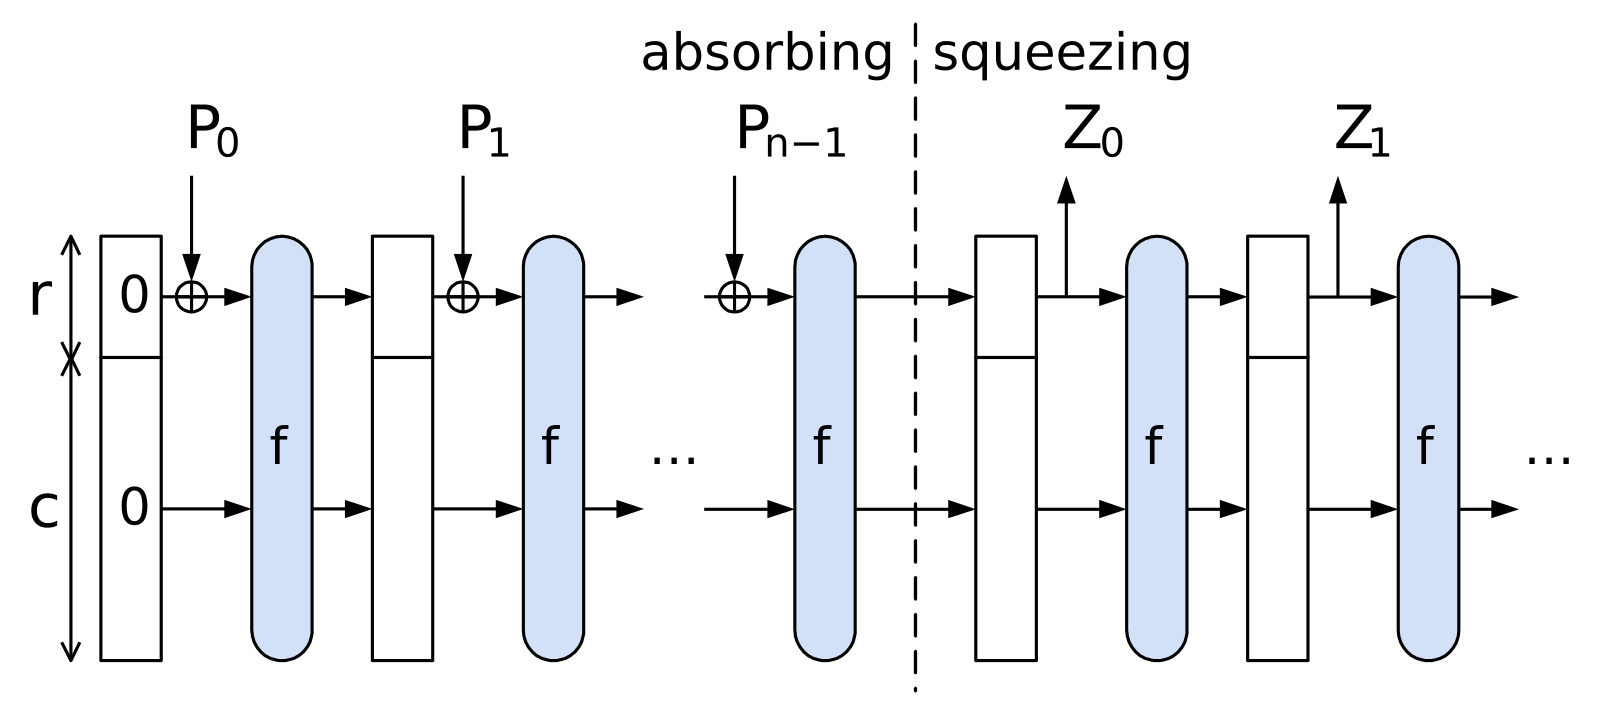
\includegraphics[width=0.8\textwidth]{sponge.png}
    \caption{Глафическое описание конструкции губки}
  \end{figure}

  \subsection{Keccak}

  Keccak - семейство криптографических хеш-функций, основанноых на структуре губки.
  Все Keccak хеш-функции обладают общей схемой выделения хеша и отличаются между
  собой только соотношением размера $r$ и $c$ (скорость к мощности) и длиной
  выходной битовой последовательности.

  Губка для таких хеш функций состоит из 1600 бит (200 байт) и часто представляется
  в виде матрицы 64-битных чисел с размером $5\times 5$. Если каждое число представить
  в виде вектора из 64 бит, то получится трёхмерное про-странство $\left(5, 5, 64\right)$.

  Что в этом пространстве принадлежит $r$, а что $c$, и какая $f$ для него опре-делена
  как раз и определяет стандарт Keccak.

  \subsubsection{Координаты и индексы}

  Бит в губке может иметь индекс $i$ от $0$ до $1599$ включительно. Этот индекс
  может быть напрямую переведён в трёхмерные координаты по формулам:

  \begin{align}
    x &= (i / 64) \bmod 64 \\
    y &= i / 64 / 64 \\
    z &= i \bmod 64
  \end{align}

  Аналогично координаты могут быть переведены в индекс:
  \begin{equation}
    i = (5 * y + x) * 6 + z
  \end{equation}

  Таким образом при впитывании происходит сложение первых $r$ бит
  сос-тояния $S$ и входных данных по модулю два, то есть имеющих
  индексы от $0$ до $r - 1$ включительно.

  \subsubsection{Преобразования состояния}

  Операция $f$ для преобразования состояния $S$ при впитывании и выжима-нии
  состоит из 24 раундов. Каждый раунд представляет из себя
  последователь-ное применении одной из 5 операций над результатом другой:
  \begin{equation}
    S_n = \iota(\chi(\pi(\rho(\theta(S_{n - 1})))), r_i)
  \end{equation}

  Здесь $r_i$ - это индекс раунда.

  Пусть $S$ - состояние губки, представляющее из себя ранее введённое
  трёх-мерное пространство размера $(5, 5, 64)$, введём на нём все перечисленные
  опе-рации ($A$ - состояние, передаваемое операции на вход, $B$ - получаемое
  на вы-ходе):
  \begin{enumerate}
    \item {
      Шаг $\theta(A)$

      Введём две дополнительные операции:
      \begin{align}
        C(i, k) &= A[i, 0, k] \oplus A[i, 1, k] \oplus A[i, 2, k] \oplus A[i, 3, k] \oplus A[i, 4, k] \\
        D(i, k) &= C((i - 1)\bmod 5, k) \oplus C((i + 1)\bmod 5, (k - 1)\bmod 64)
      \end{align}

      Тогда:
      \begin{equation}
        B[x, y, z] = A[x, y, z] \oplus D(x, z)
      \end{equation}
    }
    \item {
      Шаг $\rho(A)$

      Пусть для всех целых $z \in [0; 63] B[0, 0, z] = A[0, 0, 0]$.

      Далее пусть $x = 1$, $y = 0$, тогда для всех целых $t \in [0; 23]$:
      \begin{enumerate}
        \item Для всех целых $z \in [0; 63]$\\$B[x, y, z] = A[x, y, (z - (t + 1)\times (t + 2) / 2)\bmod 64]$
        \item $(x, y) = (y, (2x + 3y)\bmod 5)$
      \end{enumerate}
    }
    \item {
      Шаг $\pi(A)$
      \begin{equation}
        B[x, y, z] = A[(x + 3y)\bmod 5, x, z]
      \end{equation}
    }
    \item {
      Шаг $\chi(A)$
      \begin{equation}
        B[x, y, z] = A[x, y, z] \oplus ((A[(i + 1)\bmod 5, y, z] \oplus 1) \cdot A[(x + 2)\bmod 5, y, z])
      \end{equation}
    }
    \item {
      Шаг $\iota(A, r)$

      Введём дополнительную функцию $rc(t)$:
      Если $t\bmod 255 = 0$, то $rc(t) = 1$ \\
      Иначе пусть $R = [1, 0, 0, 0, 0, 0, 0]$\\
      Тогда для всех целых $i \in [1, t\bmod 255]$:
      \begin{align}
        R &= [0] + R\\
        R[0] &= R[0] \oplus R[8] \\
        R[4] &= R[4] \oplus R[8] \\
        R[5] &= R[5] \oplus R[8] \\
        R[6] &= R[6] \oplus R[8] \\
        R &= [R[0], R[1], R[2], R[3], R[4], R[5], R[6], R[7]]
      \end{align}
      $rc(t) = R[0]$\\
      Тогда пусть $RC$ - массив из 64 нулей. Для всех целых $i \in [0, 6]$\\ $RC[2^i - 1] = rc(i + 7r)$.
      Также пусть $B[x, y, z] = A[x, y, z]$, а затем для всех целых $z \in [0, 64]$
      $B[0, 0, z] = B[0, 0, z] \oplus RC[z]$
    }
  \end{enumerate}

  \subsection{Конкретные реализации SHA3}

  Различные реализации хеш-функций семейства Keccak отличаются всего несколькими параметрами:
  \begin{table}[H]
    \centering
    \begin{tabular}{|c|c|c|c|}
      \hline
      Хеш-функция & Rate, бит & Capacity, бит & Длина выхода, бит \\
      \hline
      SHA3-224 & 1152 & 548 & 224 \\
      \hline
      SHA3-256 & 1088 & 512 & 256 \\
      \hline
      SHA3-384 & 832 & 768 & 384 \\
      \hline 
      SHA3-512 & 576 & 1024 & 215 \\
      \hline
    \end{tabular}
  \end{table}

  \newpage
  \section{Программная реализация}

  Код написан на языке программирования $C++$ без использования сторон-них математических
  библиотек. Из внешенго кода используются только $format$ и $argparse$ для
  форматированного вывода и парсинга входных аргументов.

  Реализована общая структура гугбки - class TSponeStructure и общий шаб-лон 
  для Keccak хеш-функций. Также из наиболее примечательных деталей ре-ализации -
  $IBitStream$. Это интерфейс для работы с потоками бит. На их осно-ве реализован
  padding алгоритм и обогащение сообщения для хеширования дополнительными битами
  в начале и конце (по стандарту SHA3).

  При помощи входных аргументов можно указать вход (файл или другой аргумент)
  и необходимую хеш функцию.

  Результат работы моей реализации сравнивался с эталонными значениями из
  общего стандарта.

  \newpage
  \section{Демонстрация работы}

  \begin{figure}[H]
    \centering
    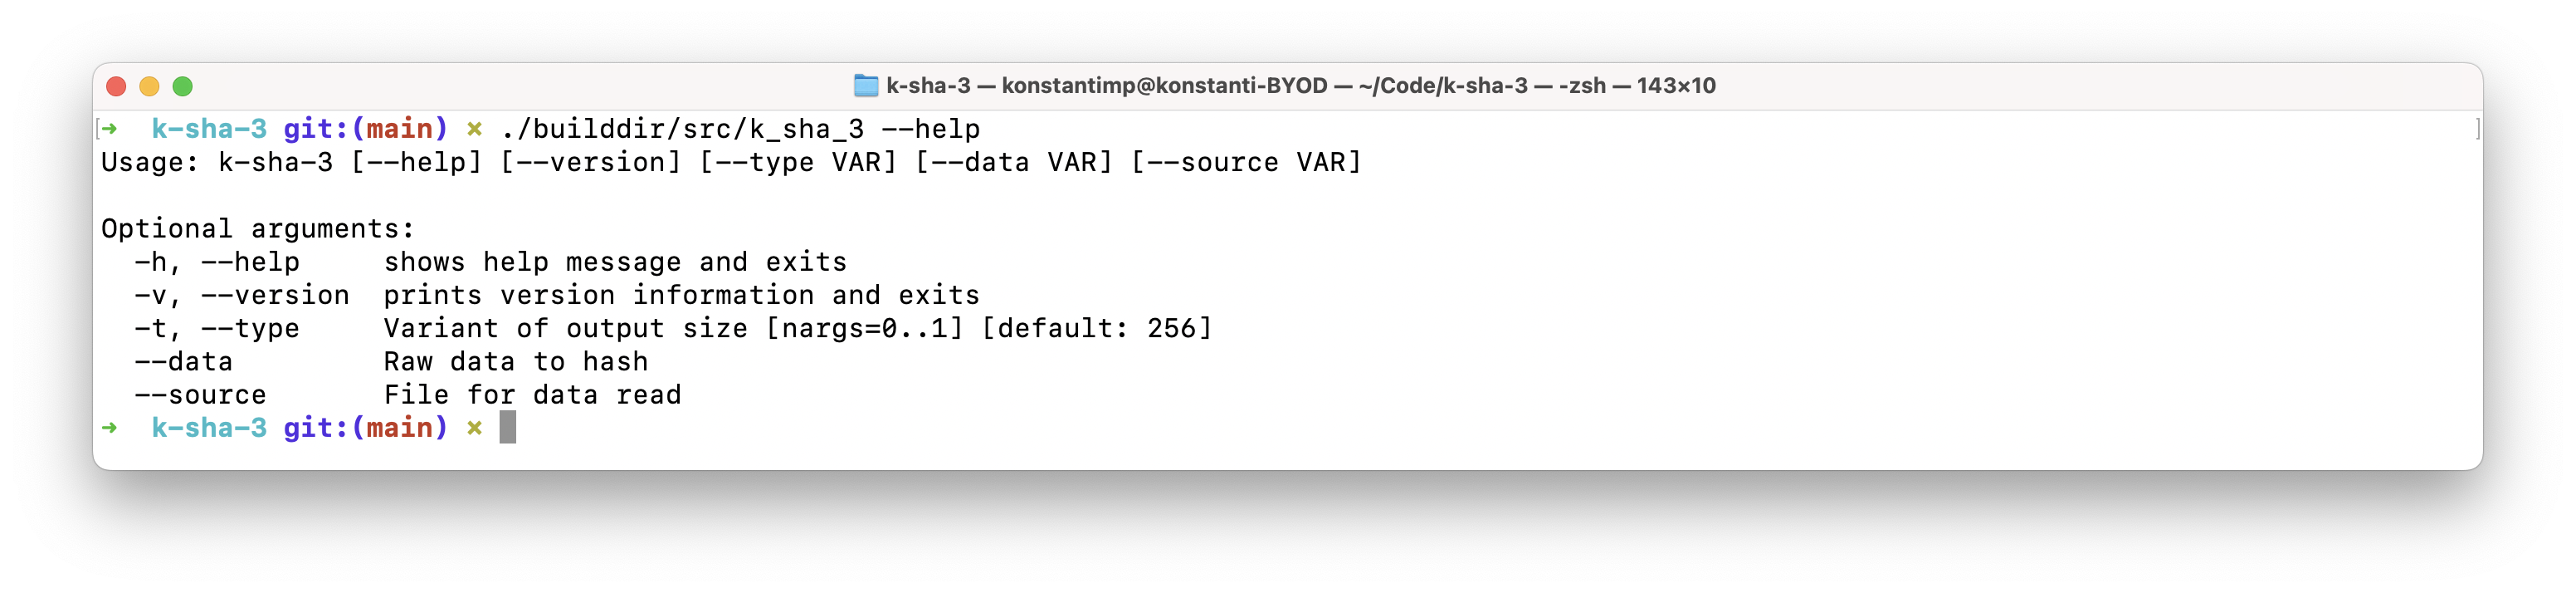
\includegraphics[width=0.8\textwidth]{sha3_1.png}
    \caption{Помощь}
  \end{figure}

  \begin{figure}[H]
    \centering
    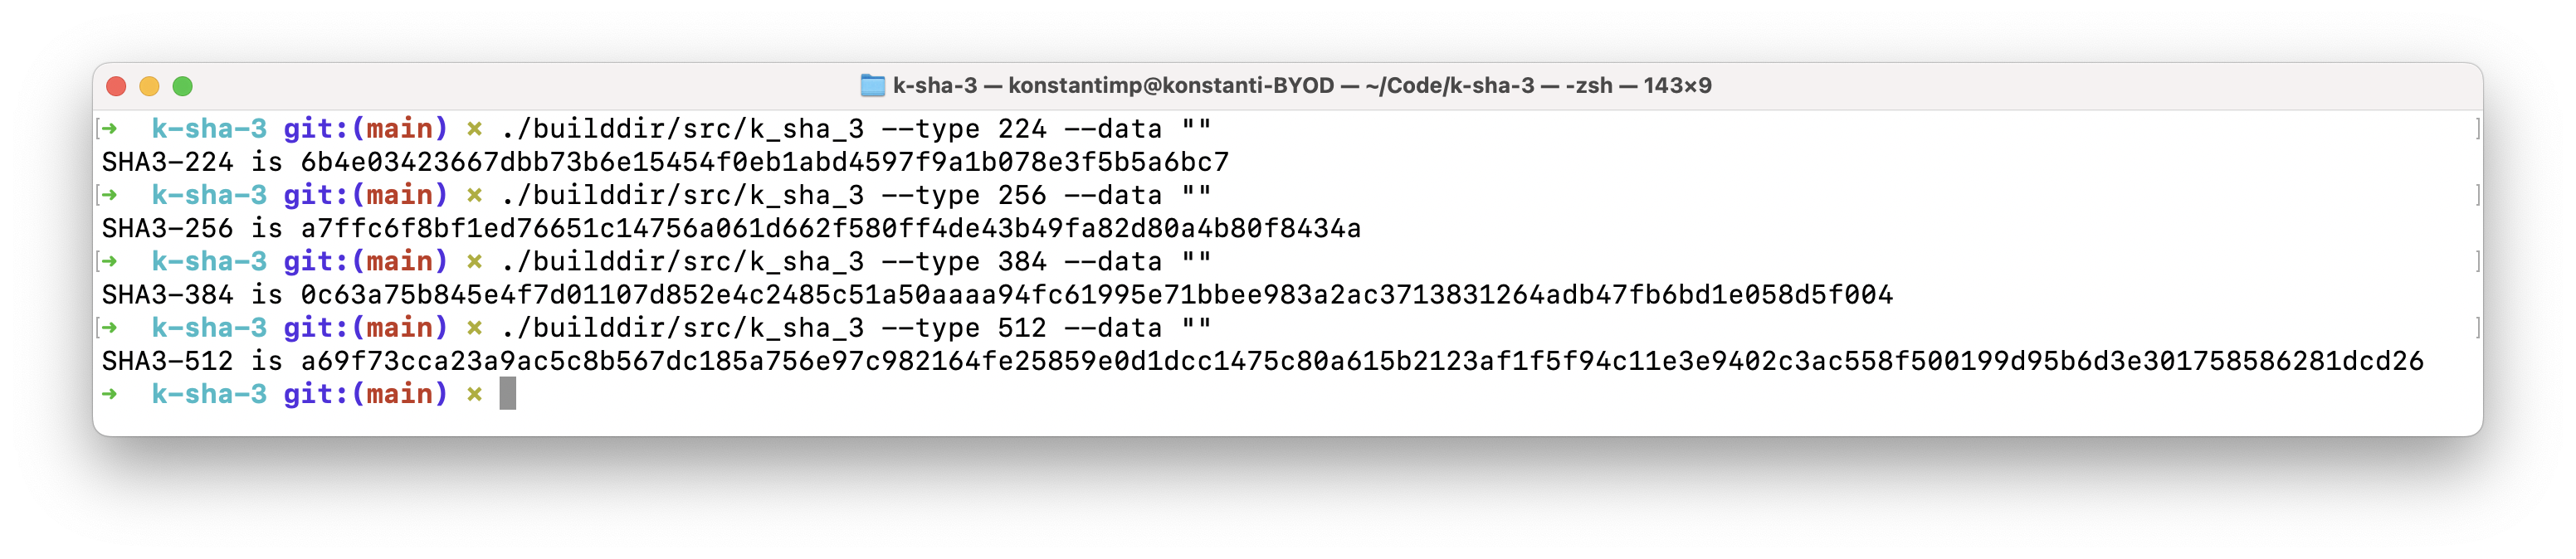
\includegraphics[width=0.8\textwidth]{sha3_2.png}
    \caption{Хеширование пустой строки}
  \end{figure}

  \begin{figure}[H]
    \centering
    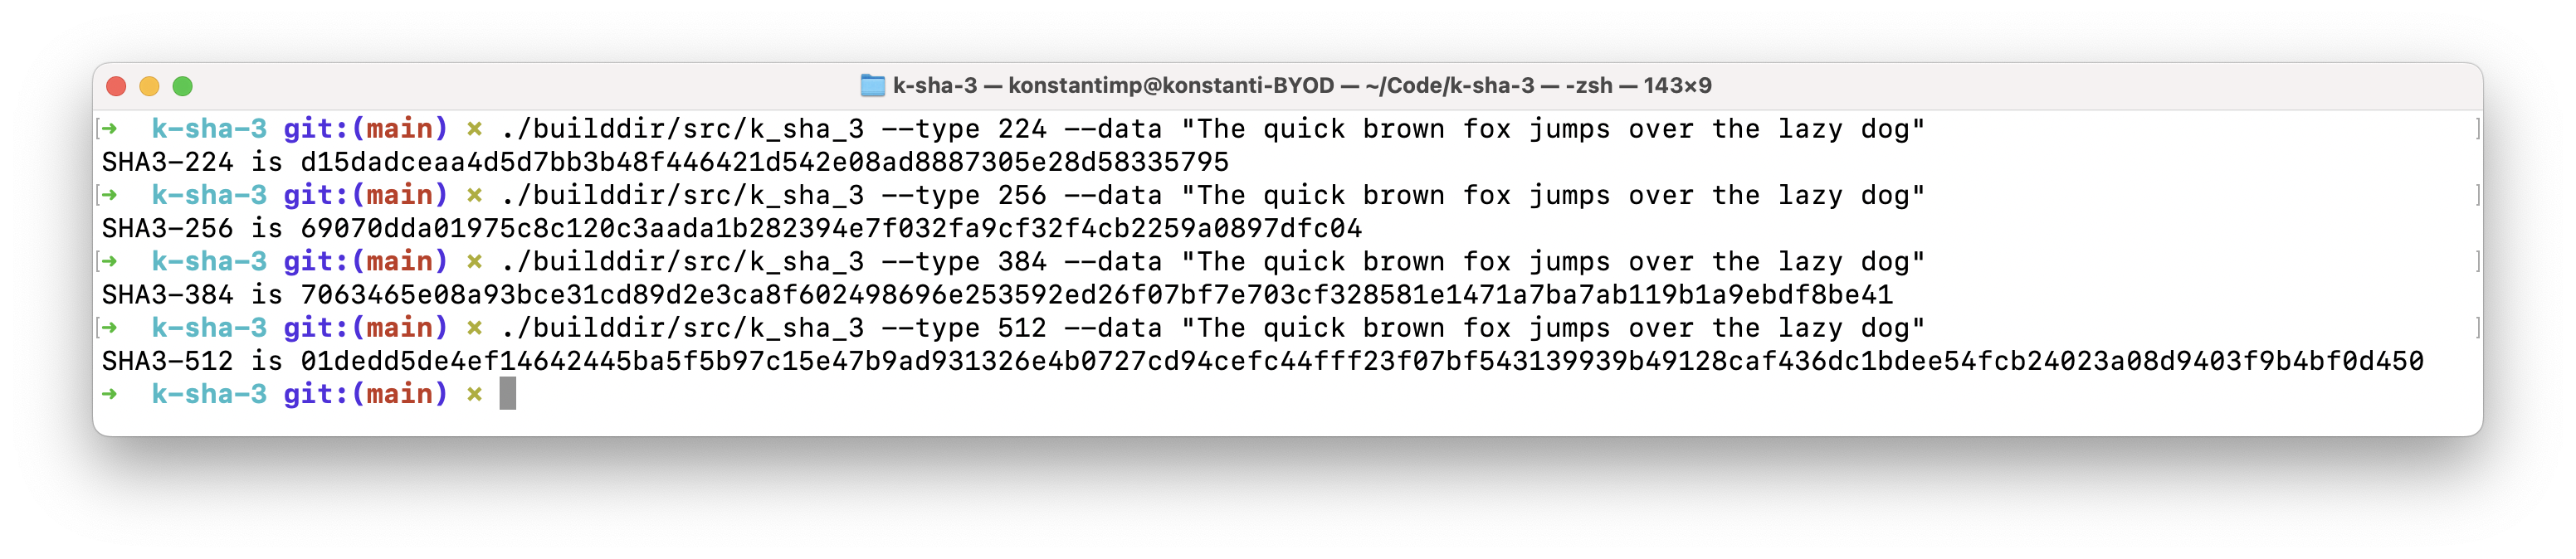
\includegraphics[width=0.8\textwidth]{sha3_3.png}
    \caption{Хеширование непустой строки}
  \end{figure}

  \newpage
  \section{Выводы}
  
  В ходе данной работы была реализована структура криптографической губки
  и основанные на ней алгоритмы хеширования.

\end{document}
